\newpage
\Author{Autor: \daAuthorThree}


\section{Noch ein paar Zitate}



Das ist der Text, welcher zitiert werden soll  \autocite{HTL-Kaindorf-2},
leider gibt es kein Erscheinungsdatum für diese Seite (stimmt nicht, könnte aber passieren). Das Zugriffsdatum wurde unter \anf{urldate} in der Datei \anf{references.bib} eingegeben.

\begin{longcite}
	\anf{Führt man einem Stoff Energie in Form von Wärme 
		zu, so dehnt er sich nach allen Seiten aus. Diese Volumenvergrößerung ist eine Folge der Vergrößerung 
		des mittleren Abstandes der Stoffteilchen untereinander. Bei Abkühlung zeigt sich eine entsprechende 
		Volumenabnahme. 
		Die Größe der Wärmeausdehnung hängt von der Art 
		des Stoffes ab. Feste Körper dehnen sich nur wenig, 
		Flüssigkeiten dagegen stärker aus. Die größte Ausdehnung zeigt sich bei den Gasen. } \autocite[F9]{Boege2011}
\end{longcite}

Das ist die Textpassage, welche nicht wörtlich zitiert werden soll \autocite[vgl.][399]{einstein}, und noch einmal ohne Seitenangabe \autocite[vgl.][]{einstein}.
Man kann auch Tabellen zitieren: \autocite[vgl.][Tab. 2]{einstein}.

\autocite[Tab. 8.1]{Decker2018}

\section{Mathematische Ausdrücke}
\subsection{Formeln}
\begin{equation}
	\label{eq:1}
	\int\limits_{a}^{b} x^{2} \, dx = \frac{ b^{3} - a^{3} }{3}
\end{equation}

\begin{equation}
	\label{eq:pythagoras}
	c = \sqrt{ a^{2} + b^{2} }
\end{equation}

Die Formel des Pythagoras wird in Gleichung (\ref{eq:pythagoras}) angegeben.

\subsection{SI-Einheiten}

SI-Einheiten werden mit dem Befehl \verb|\si{}| erstellt. Die Eingabe \verb|$[F] = \si{\newton}$| ergibt 

$[F] = \si{\newton}$,

\verb|$[I]=\si{\mm\tothe{4}}$|

$[I]=\si{\mm\tothe{4}}$.

Werden Einheiten öfter verwendet, ist es sinnvoll, diese vorher mittels \verb|\newcommand{}| zu definieren.
 Die Definition befindet sich in diesem Beispiel in der Datei \anf{SH/common\_things.tex}. 
 
\begin{verbatim}
	\newcommand{\esigma}{\ensuremath{\si[per-mode=fraction]...
	...{\newton\per\mm\squared}}}
\end{verbatim}

Die Eingabe für eine mechanische Spannung sieht dann beispielsweise so aus:

\verb|$\sigma_1=500\esigma$|.

$\sigma_1=500\esigma$ 

Auflistung der standardmäßigen Einheiten und weitere Informationen findet man unter \url{https://www.namsu.de/Extra/pakete/Siunitx.html}


\section{Fortsetzung}

\subsection{Unterkapitel des Textes}
So sieht die Formatierung eines Unterkapitels aus.
Weiter geht es mit einer neuen Seite.

\newpage

\subsubsection{Unterunterkapitel ;-)}
Dieses Unterunterkapitel bekommt einen eigene Seite.

Ein Foto der Schule darf auch nicht fehlen. Die Quellenangabe ist noch in Arbeit.


	
\begin{figure}[htb]
	\centering
	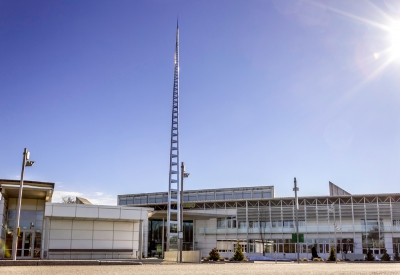
\includegraphics[width=0.8\linewidth]{images/thumb-htlkaindorf_1-bf57c0aa8b00a13c9a8b98cc8bea49f0.jpg}
	\caption{Die schönste Schule}
	\label{fig:diag1}
\end{figure}

\subsection{Einstellungsmöglichkeiten in diesem Dokumentes}
In der Datei \anf{da-defines.tex} können einige Voreinstellungen festgelegt werden:
\begin{itemize}
	\item die Abteilungsspezifische Titelseitenvorlage
	\item die Dokumentsprache
	\item doppelseitiges Drucken
	\item Schrift mit oder ohne Serifen
\end{itemize}

\subsection{Individuelle Daten für die Diplomarbeit}
Des Weiteren können in der Datei  \anf{da-defines.tex} die Angaben zur Diplomarbeit, die Namen der Schüler sowie der schulinterner und externer Betreuer eingegeben werden.


Listen für Literatureinträge können in der Datei \anf{da-0.0\_mainDocument.tex} im Bereich \anf{Referenz-Liste(n) der zu zitierenden Litatur} ergänzt/geändert werden.



\subsection{Probleme im Dokument}
Bei langen Autornamen und langem Diplomarbeitstitel gibt es eine Kollision in der Fußzeile.